%%%%%%%%%%%%%%%%%%%%%%%%%%%%%%%%%%%%%%%%%
% Beamer Presentation
% LaTeX Template
% Version 1.0 (10/11/12)
%
% This template has been downloaded from:
% http://www.LaTeXTemplates.com
%
% License:
% CC BY-NC-SA 3.0 (http://creativecommons.org/licenses/by-nc-sa/3.0/)
%
%%%%%%%%%%%%%%%%%%%%%%%%%%%%%%%%%%%%%%%%%

%----------------------------------------------------------------------------------------
%	PACKAGES AND THEMES
%----------------------------------------------------------------------------------------

\documentclass{beamer}

\mode<presentation> {

% The Beamer class comes with a number of default slide themes
% which change the colors and layouts of slides. Below this is a list
% of all the themes, uncomment each in turn to see what they look like.

%\usetheme{default}
%\usetheme{AnnArbor}
%\usetheme{Antibes}
%\usetheme{Bergen}
%\usetheme{Berkeley}
%\usetheme{Berlin}
%\usetheme{Boadilla}
%\usetheme{CambridgeUS}
%\usetheme{Copenhagen}
%\usetheme{Darmstadt}
%\usetheme{Dresden}
%\usetheme{Frankfurt}
%\usetheme{Goettingen}
%\usetheme{Hannover}
%\usetheme{Ilmenau}
%\usetheme{JuanLesPins}
%\usetheme{Luebeck}
\usetheme{Madrid}
% \usetheme{Malmoe}
%\usetheme{Marburg}
%\usetheme{Montpellier}
%\usetheme{PaloAlto}
%\usetheme{Pittsburgh}
%\usetheme{Rochester}
%\usetheme{Singapore}
%\usetheme{Szeged}
%\usetheme{Warsaw}

% As well as themes, the Beamer class has a number of color themes
% for any slide theme. Uncomment each of these in turn to see how it
% changes the colors of your current slide theme.

%\usecolortheme{albatross}
%\usecolortheme{beaver}
%\usecolortheme{beetle}
%\usecolortheme{crane}
%\usecolortheme{dolphin}
%\usecolortheme{dove}
%\usecolortheme{fly}
%\usecolortheme{lily}
%\usecolortheme{orchid}
%\usecolortheme{rose}
%\usecolortheme{seagull}
%\usecolortheme{seahorse}
%\usecolortheme{whale}
%\usecolortheme{wolverine}

\setbeamertemplate{footline} % To remove the footer line in all slides uncomment this line
%\setbeamertemplate{footline}[page number] % To replace the footer line in all slides with a simple slide count uncomment this line

%\setbeamertemplate{navigation symbols}{} % To remove the navigation symbols from the bottom of all slides uncomment this line
}

\usepackage{graphicx} % Allows including images
\usepackage{booktabs} % Allows the use of \toprule, \midrule and \bottomrule in tables

%----------------------------------------------------------------------------------------
%	TITLE PAGE
%----------------------------------------------------------------------------------------

\title[]{\textbf{Risk Parity Model Based on MVT}\\ DTFF Final Assignment} % The short title appears at the bottom of every slide, the full title is only on the title page

\author{\textit{Zifeng Tang(21-742-093)} \\ \textit{Yuzhi Mao(21-742-218)} \\ \textit{Haoran Zhu(21-742-069)} }
\date{Due date: 19th December 2022}
\logo{
\includegraphics[height=0.5cm]{Figure/LOGO.png}}

\begin{document}

\begin{frame}
\titlepage % Print the title page as the first slide
\end{frame}

\begin{frame}
\frametitle{Overview} % Table of contents slide, comment this block out to remove it
\tableofcontents % Throughout your presentation, if you choose to use \section{} and \subsection{} commands, these will automatically be printed on this slide as an overview of your presentation
\end{frame}

%----------------------------------------------------------------------------------------
%	PRESENTATION SLIDES
%----------------------------------------------------------------------------------------

%------------------------------------------------
\section{Introduction} % Sections can be created in order to organize your presentation into discrete blocks, all sections and subsections are automatically printed in the table of contents as an overview of the talk
%------------------------------------------------
\begin{frame}
\frametitle{Overview} % Table of contents slide, comment this block out to remove it
\tableofcontents[currentsection] % Throughout your presentation, if you choose to use \section{} and \subsection{} commands, these will automatically be printed on this slide as an overview of your presentation
\end{frame}

\subsection{Risk Measures}
\begin{frame}{Risk Measures}
Since investors pay more attention to the downside risk of financial assets, two indicators to measure the downside risk are raised.
\begin{block}{Definition 1: Mean Downside Semi Variance}
\begin{equation*}
    \text{SV}_{m} = \frac{1}{T} \sum_{t=1}^T \max \left[0, E(R_{t})-R_{t}\right]^2    
\end{equation*}
    where $E(R_{t})$ is the average rate of return.
\end{block}
\begin{block}{Definition 2: Target Downside Semi Variance}
\begin{equation*}
    \text{SV}_{t} =\frac{1}{T} \sum_{t=1}^T \max \left[0, R^*-R_t\right]^2    
\end{equation*}
    where $R^*$ is the target rate of return.
\end{block}
\end{frame}

\begin{frame}{Risk Measures}
Besides the risk metrics, there are three indicators to measure value at risk.
\begin{block}{Definition 3: Value at Risk}
\begin{equation*}
\operatorname{VaR}_\alpha(X)=-q_\alpha(X)=-\inf \{x: P[X \leq x] \geq \alpha\}     
\end{equation*}
where $X$ is a given random variable, and $\alpha$ is the confidence level.
\end{block}

\begin{block}{Definition 4: Conditional Value at Risk}
\begin{equation*}
\operatorname{CVaR}_\alpha(X)=-E\left[X \leq q_\alpha(X)\right]       
\end{equation*}
\end{block}

\begin{block}{Definition 5: Expected Shortfall}
\begin{equation*}
 ES(\alpha)=\frac{\int_0^\alpha \operatorname{VaR}(u) du}{\alpha}      
\end{equation*}
\end{block}

\end{frame}




\subsection{Risk Parity Model}

\begin{frame}{Risk Parity Model}
The core idea of All Weather strategy is to equates the risk of each asset by determining their weights in the asset portfolio.

\begin{block}{Definition of Total Risk $\boldsymbol{\mathcal{R}}_\mathbf{p}(\vec{w})$ of a Portfolio}
 \begin{equation*}
\boldsymbol{\mathcal{R}}_{\mathbf{p}}=\sqrt{\vec{w}^T \Sigma \vec{w}}
 \end{equation*}
\end{block}

\begin{block}{Definition of the Marginal Risk and the Risk Contribution}

\begin{itemize}
    \item \textbf{Marginal Risk $\boldsymbol{M}\boldsymbol{\mathcal{R}}(X_{i})$ of each asset $i$ of a Portfolio}\begin{equation*}\boldsymbol{M}\boldsymbol{\mathcal{R}}\left(X_i\right)=\frac{\partial \boldsymbol{\mathcal{R}}_{\mathbf{p}}}{\partial w_i}
    \end{equation*}
    \item \textbf{Risk Contribution $\boldsymbol{\mathcal{R}}\boldsymbol{C}(X_i)$ of each asset $i$ of a Portfolio}\begin{equation*}
    \boldsymbol{\mathcal{R}}\boldsymbol{C}\left(X_i\right) =w_i \frac{\partial \boldsymbol{R}_\mathbf{p}}{\partial w_i}=w_i \frac{(\Sigma \vec{w})_i}{\sqrt{\vec{w}^T \sum \vec{w}}} 
    \end{equation*}
 
 \end{itemize}

\end{block}

\end{frame}

\section{Calculate Risk Measures based on Multivariate
t-distribution (MVT)}
\begin{frame}
\frametitle{Overview} % Table of contents slide, comment this block out to remove it
\tableofcontents[currentsection] % Throughout your presentation, if you choose to use \section{} and \subsection{} commands, these will automatically be printed on this slide as an overview of your presentation
\end{frame}

\subsection{Data Description and Normality Test}
\begin{frame}
\frametitle{Data Description}
We use CSI 300, CSI Aggregate Bond Index and Gold Exchange Traded Fund to represent the performance of stock, marketable securities, and commodity markets, respectively. The following figures represent the Daily Return of CSI-300, CSI-ABI, and Gold-
ETF (lower left) and the Correlation Matrix.
\begin{figure}[H]
    \centering
    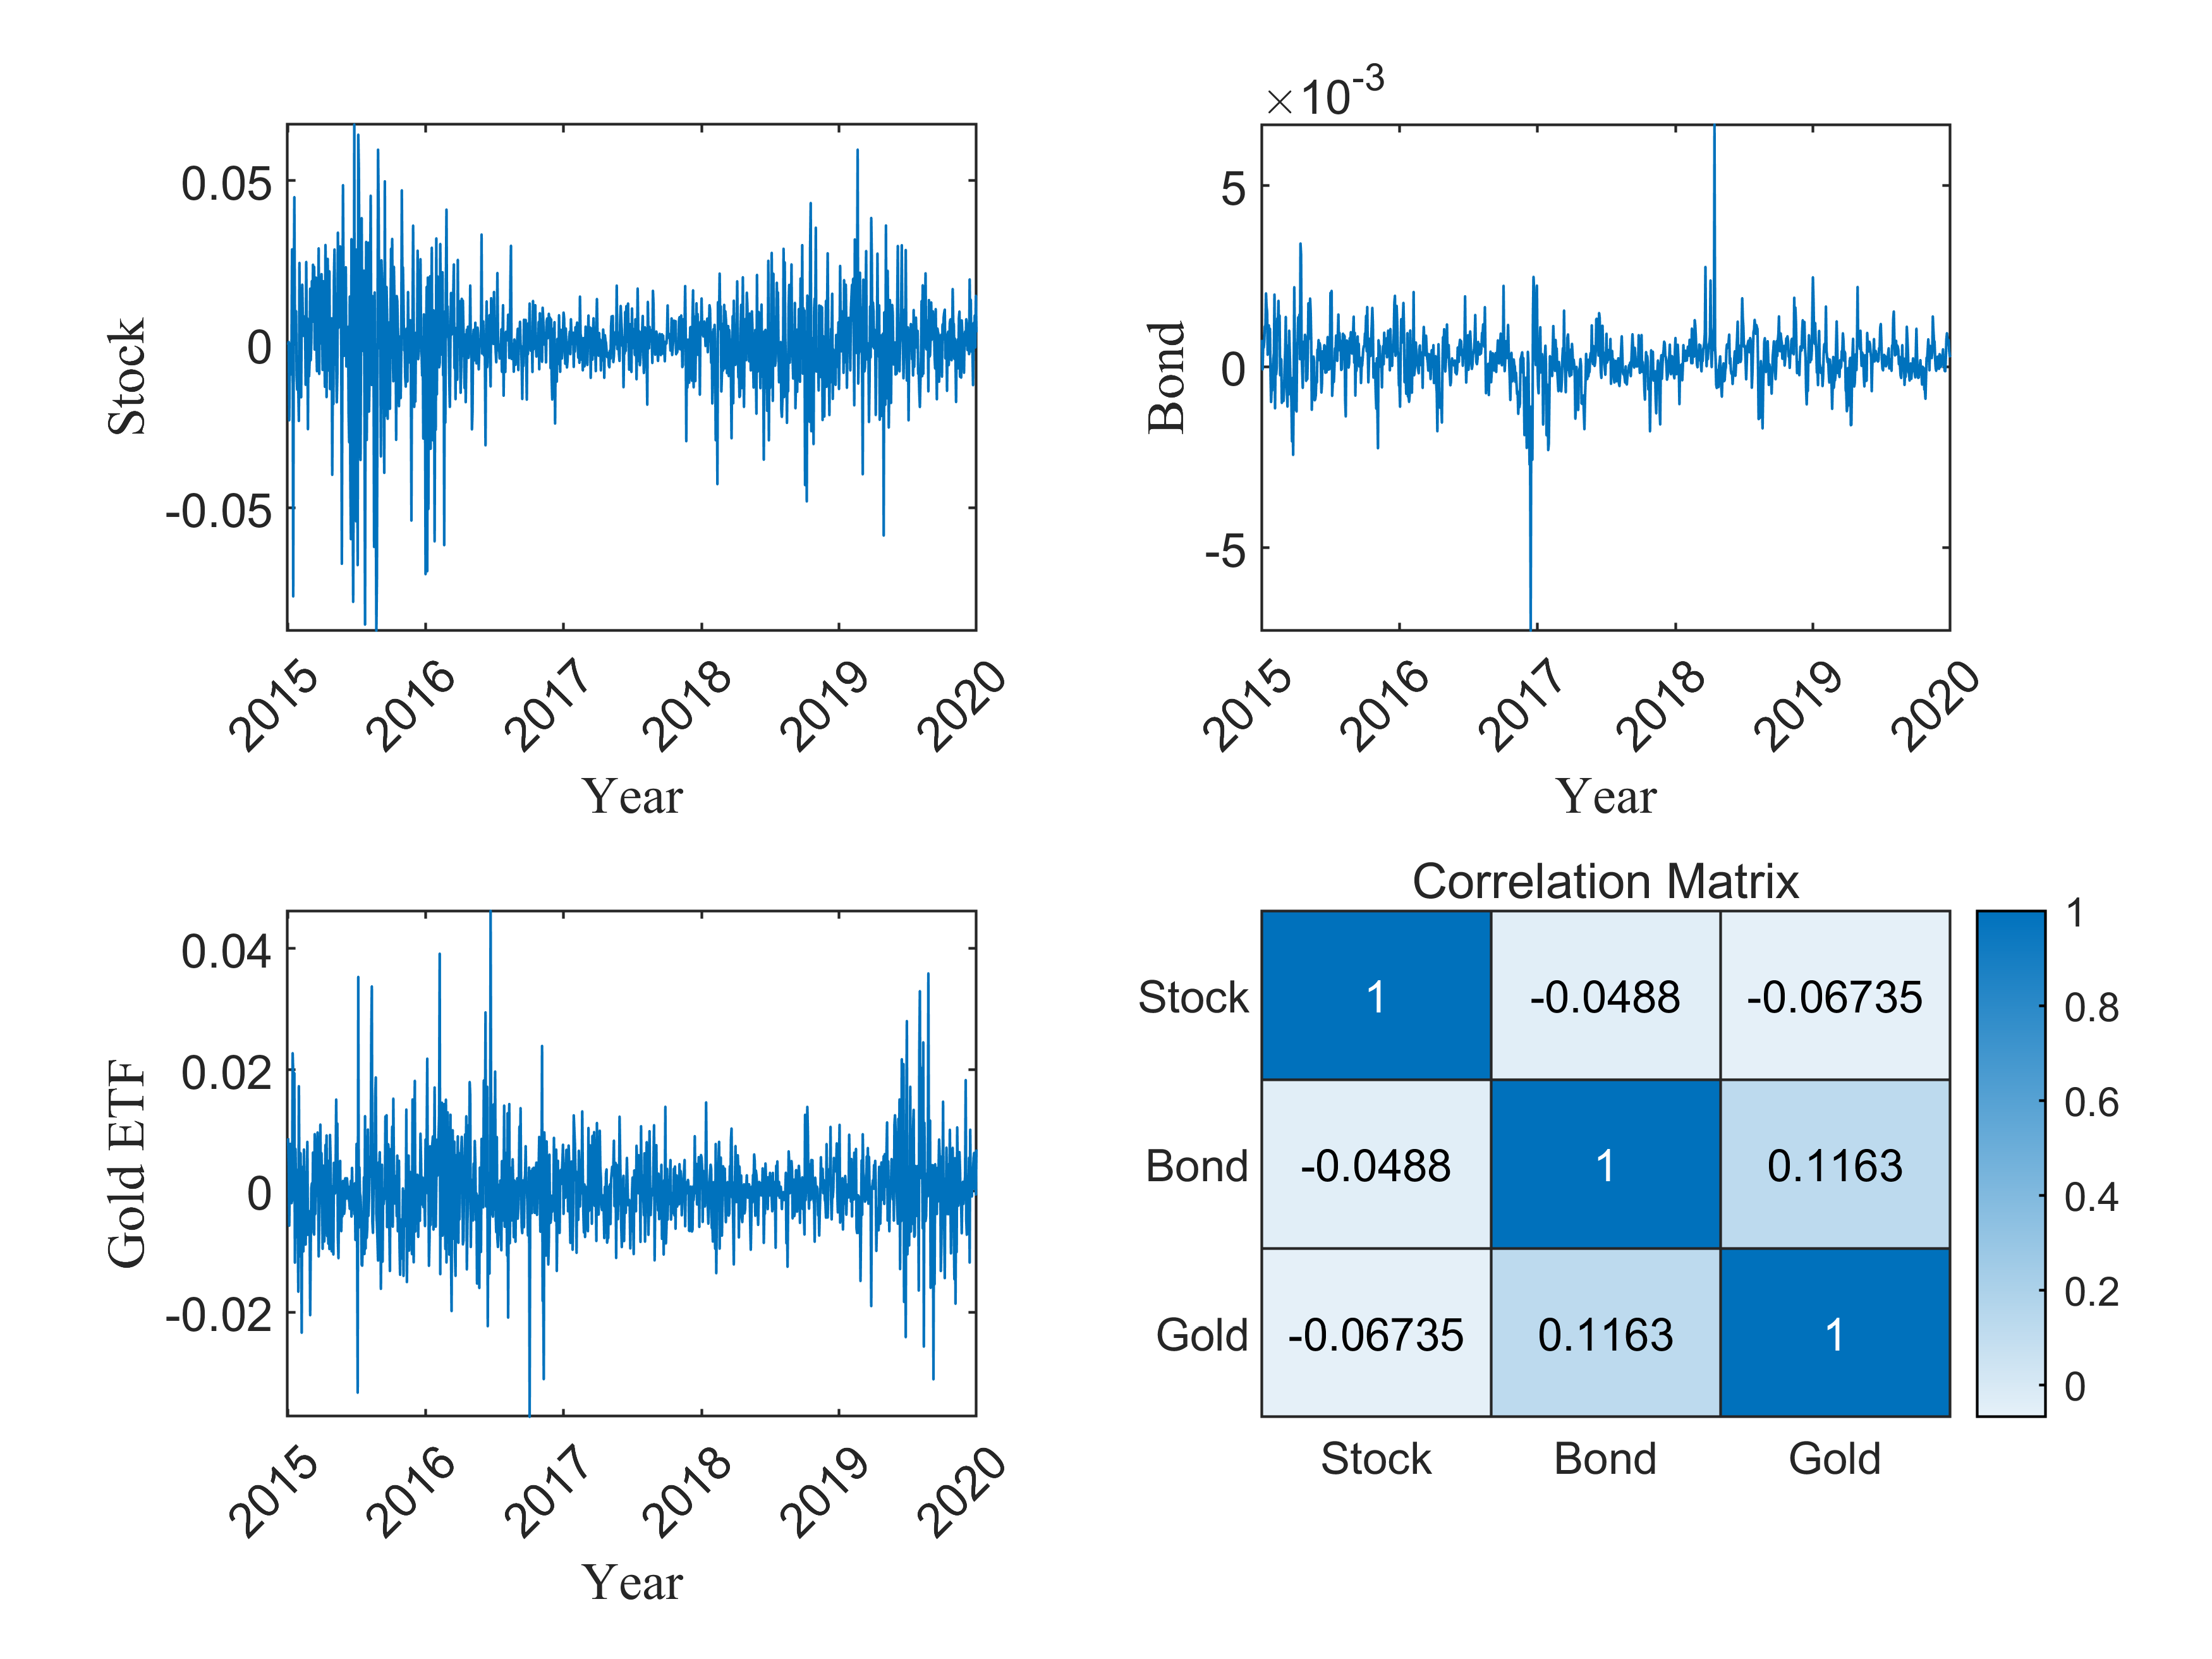
\includegraphics[scale=0.5]{Figure/FIG1-Daily-Return.png}
    \label{Fig1}
\end{figure}
% \begin{block}{Definition 1}
% \textbf{Definition}
% \begin{itemize}
%     \item[1)] 
%     \item[2)]
%     \item[3)] 
% \end{itemize}
% \end{block}
\end{frame}

\begin{frame}{Normality Test}
\begin{figure}[H]
    \centering
    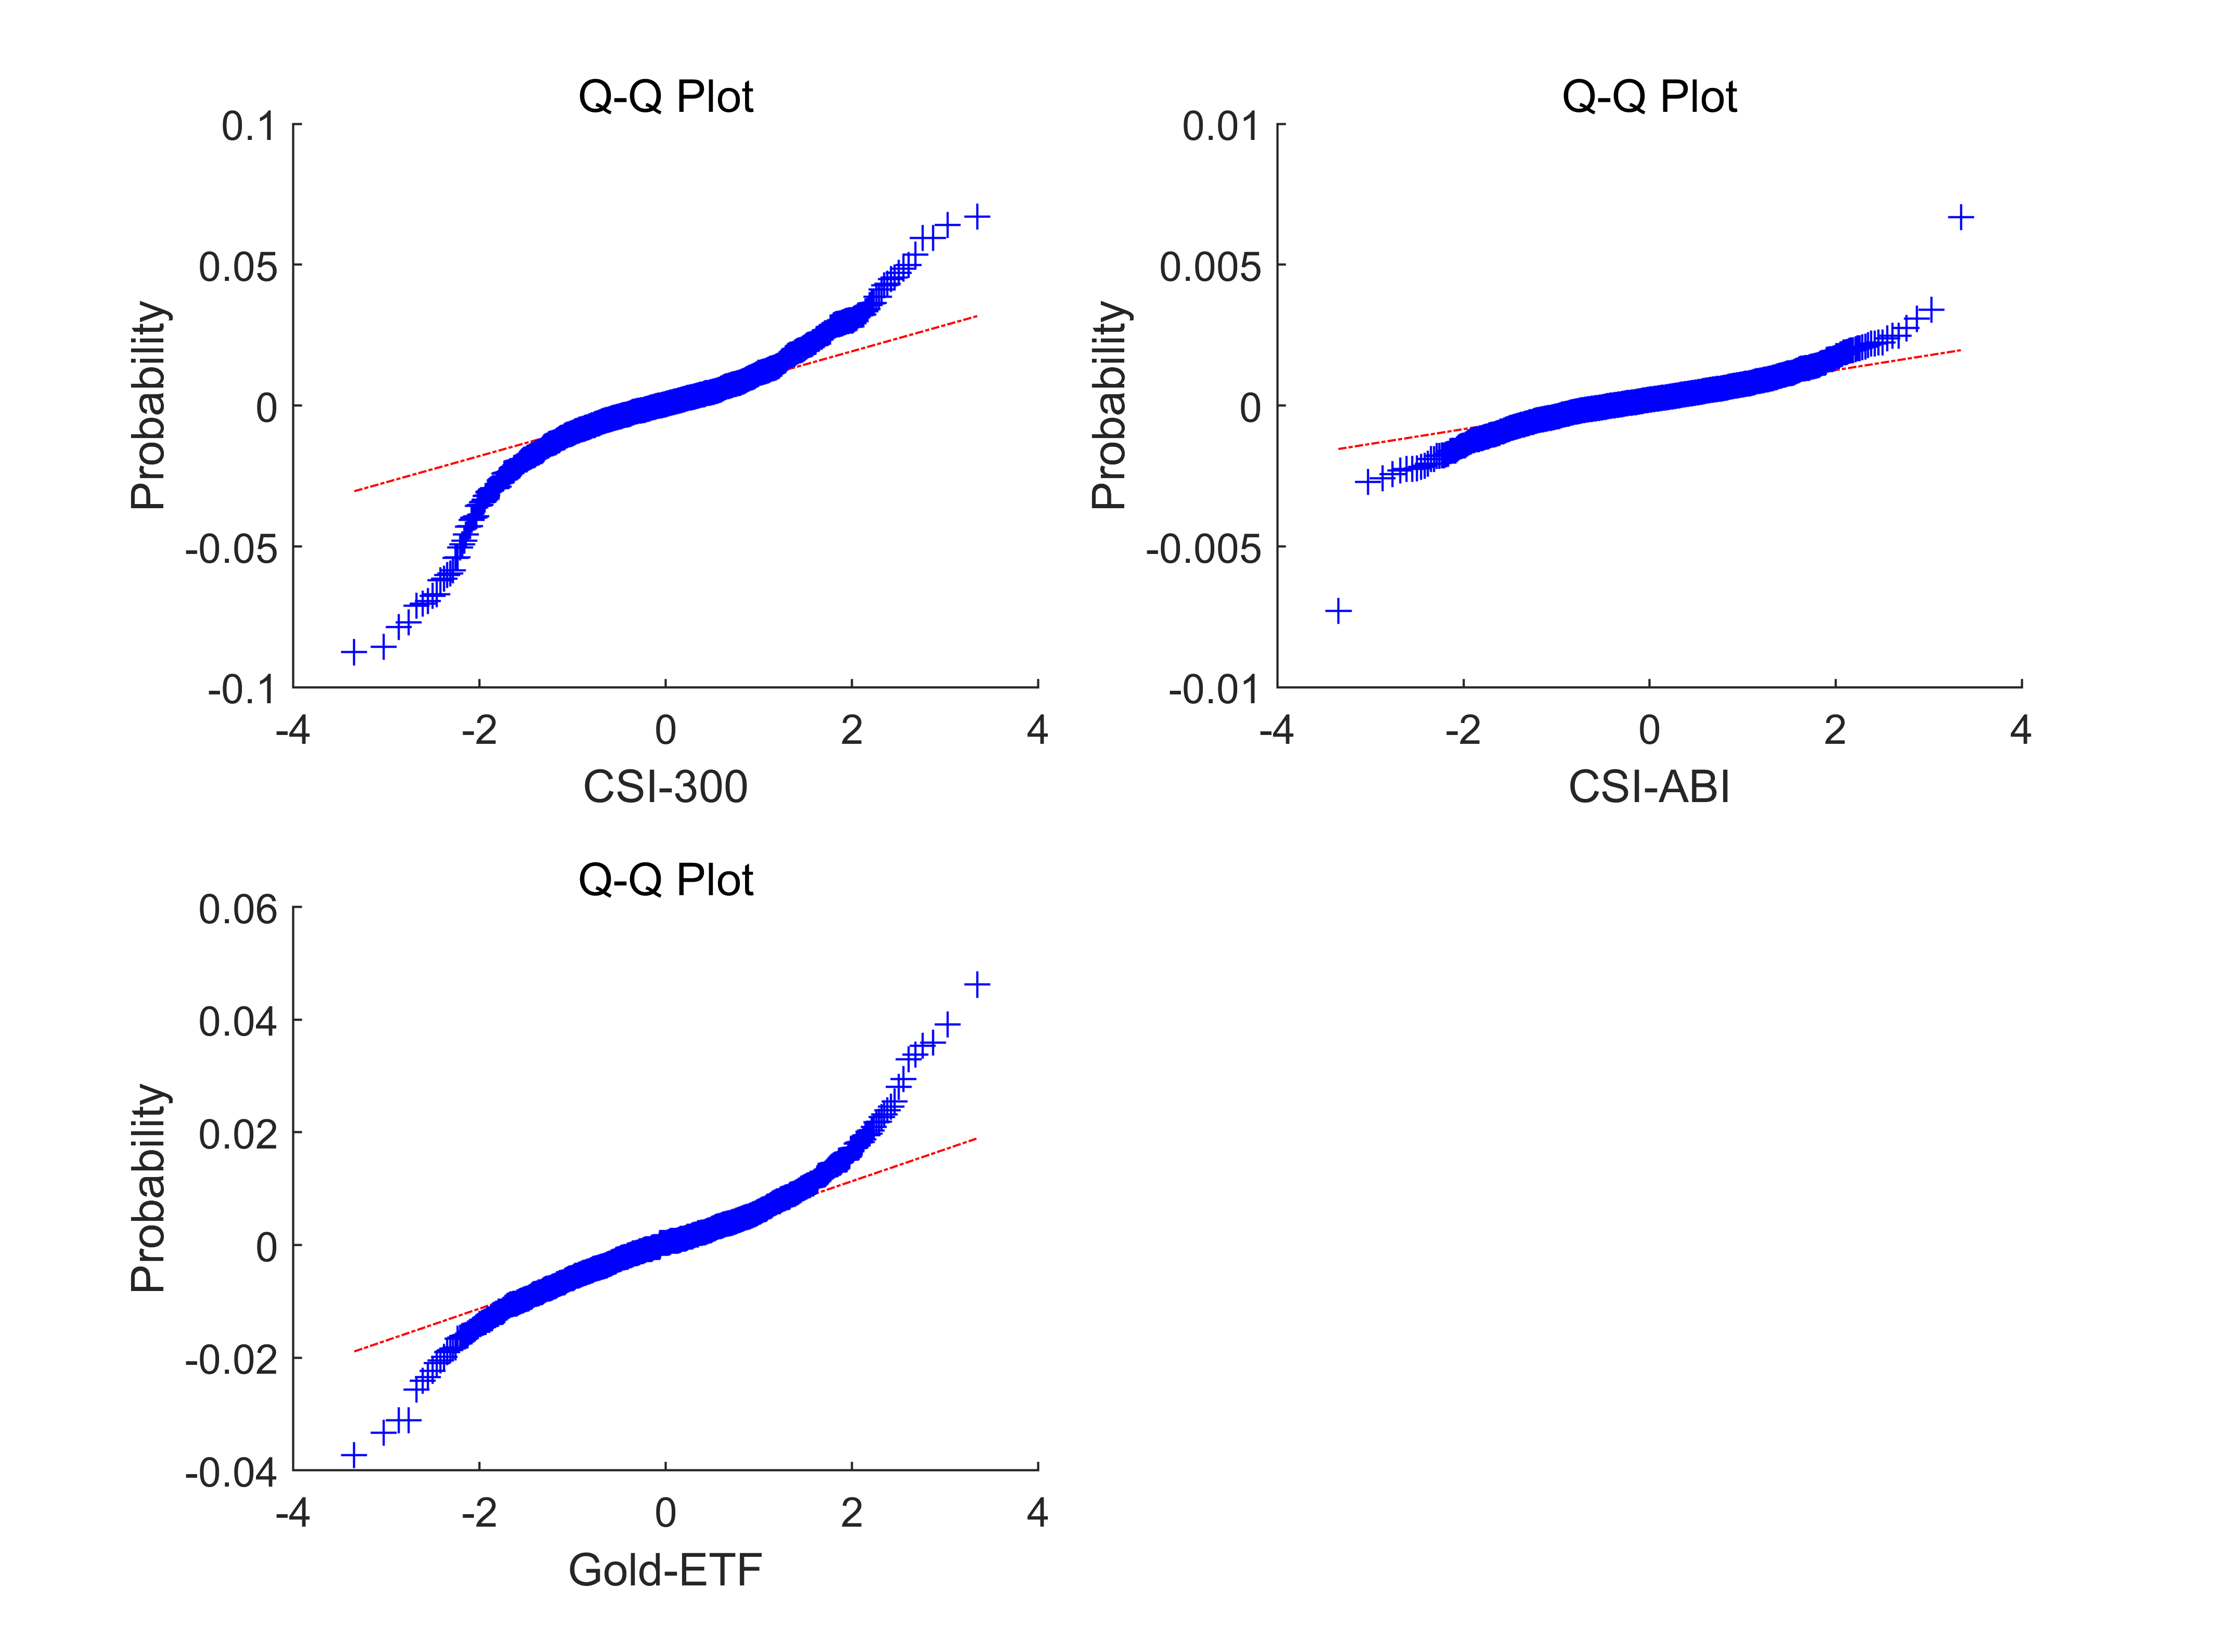
\includegraphics[scale=0.5]{Figure/FIG2-Q-Q.png}
    \label{Fig2}
\end{figure}
\end{frame}

\begin{frame}{Characteristics of the Data}
\begin{block}{Three Characteristics}
\begin{itemize}
    \item \textbf{Volatility:} The volatility of the stock market is the highest while that of the bond market is the lowest, and the volatility of the gold market is in the middle.
    \item \textbf{Leptokurtic:} All of the three types of assets have kurtosis greater than 3, and have bias. It is known as "peak and fat tail".
    \item \textbf{Normality Test:} From the Q-Q plot, it is clear that the logarithmic return of the three assets does not follow the normal distribution. 
\end{itemize}
\end{block}

\end{frame}



\subsection{Parameter Estimation of MVT Distribution}

\begin{frame}{Parameter Estimation of MVT Distribution}
Since the normal distribution is not effective to describe the return
on financial assets, so we introduce the multivariate t distribution (MVT). 

\begin{block}{Density Function of d-dimensional Student t Distribution $T_\nu(\mu, \Sigma)$}
\begin{equation*}\label{E1.1}
p(x \mid v, \mu, \Sigma)=\frac{\Gamma\left(\frac{d+v}{2}\right)}{\Gamma\left(\frac{v}{2}\right) v^{\frac{d}{2}} \pi^{\frac{d}{2}}|\Sigma|^{\frac{1}{2}}} \frac{1}{\left(1+\frac{1}{v}(x-\mu)^{\mathrm{T}} \Sigma^{-1}(x-\mu)\right)^{\frac{d+v}{2}}}
\end{equation*} 
with $v>$ 0 degrees of freedom, location paramter $\mu \in \mathbb{R}^d$ and symmetric, positive definite scatter matrix $\Sigma \in \operatorname{SPD}(\mathrm{d})$ 
\end{block}
    
\end{frame}
\begin{frame}{Parameter Estimation of MVT Distribution}
Through the MMF method, we obtain the estimated parameters
$$
\hat{\nu}=3.4273,\:\hat{\mu}=[8.519,1.783,2.064]\times 10^{-4}
$$
$$
\hat{\Sigma}=\begin{bmatrix}
  998 &  -2.55 &  -7.24 \\
 -2.55 &   2.59 &   3.25 \\
 -7.24 &   3.25 &   279 \\    
\end{bmatrix} \times 10^{-7}
$$
\end{frame}

\begin{frame}{Parameter Estimation of MVT Distribution}
Using the estimated parameters, we draw the probability density function. 
\begin{figure}[H]
    \centering
    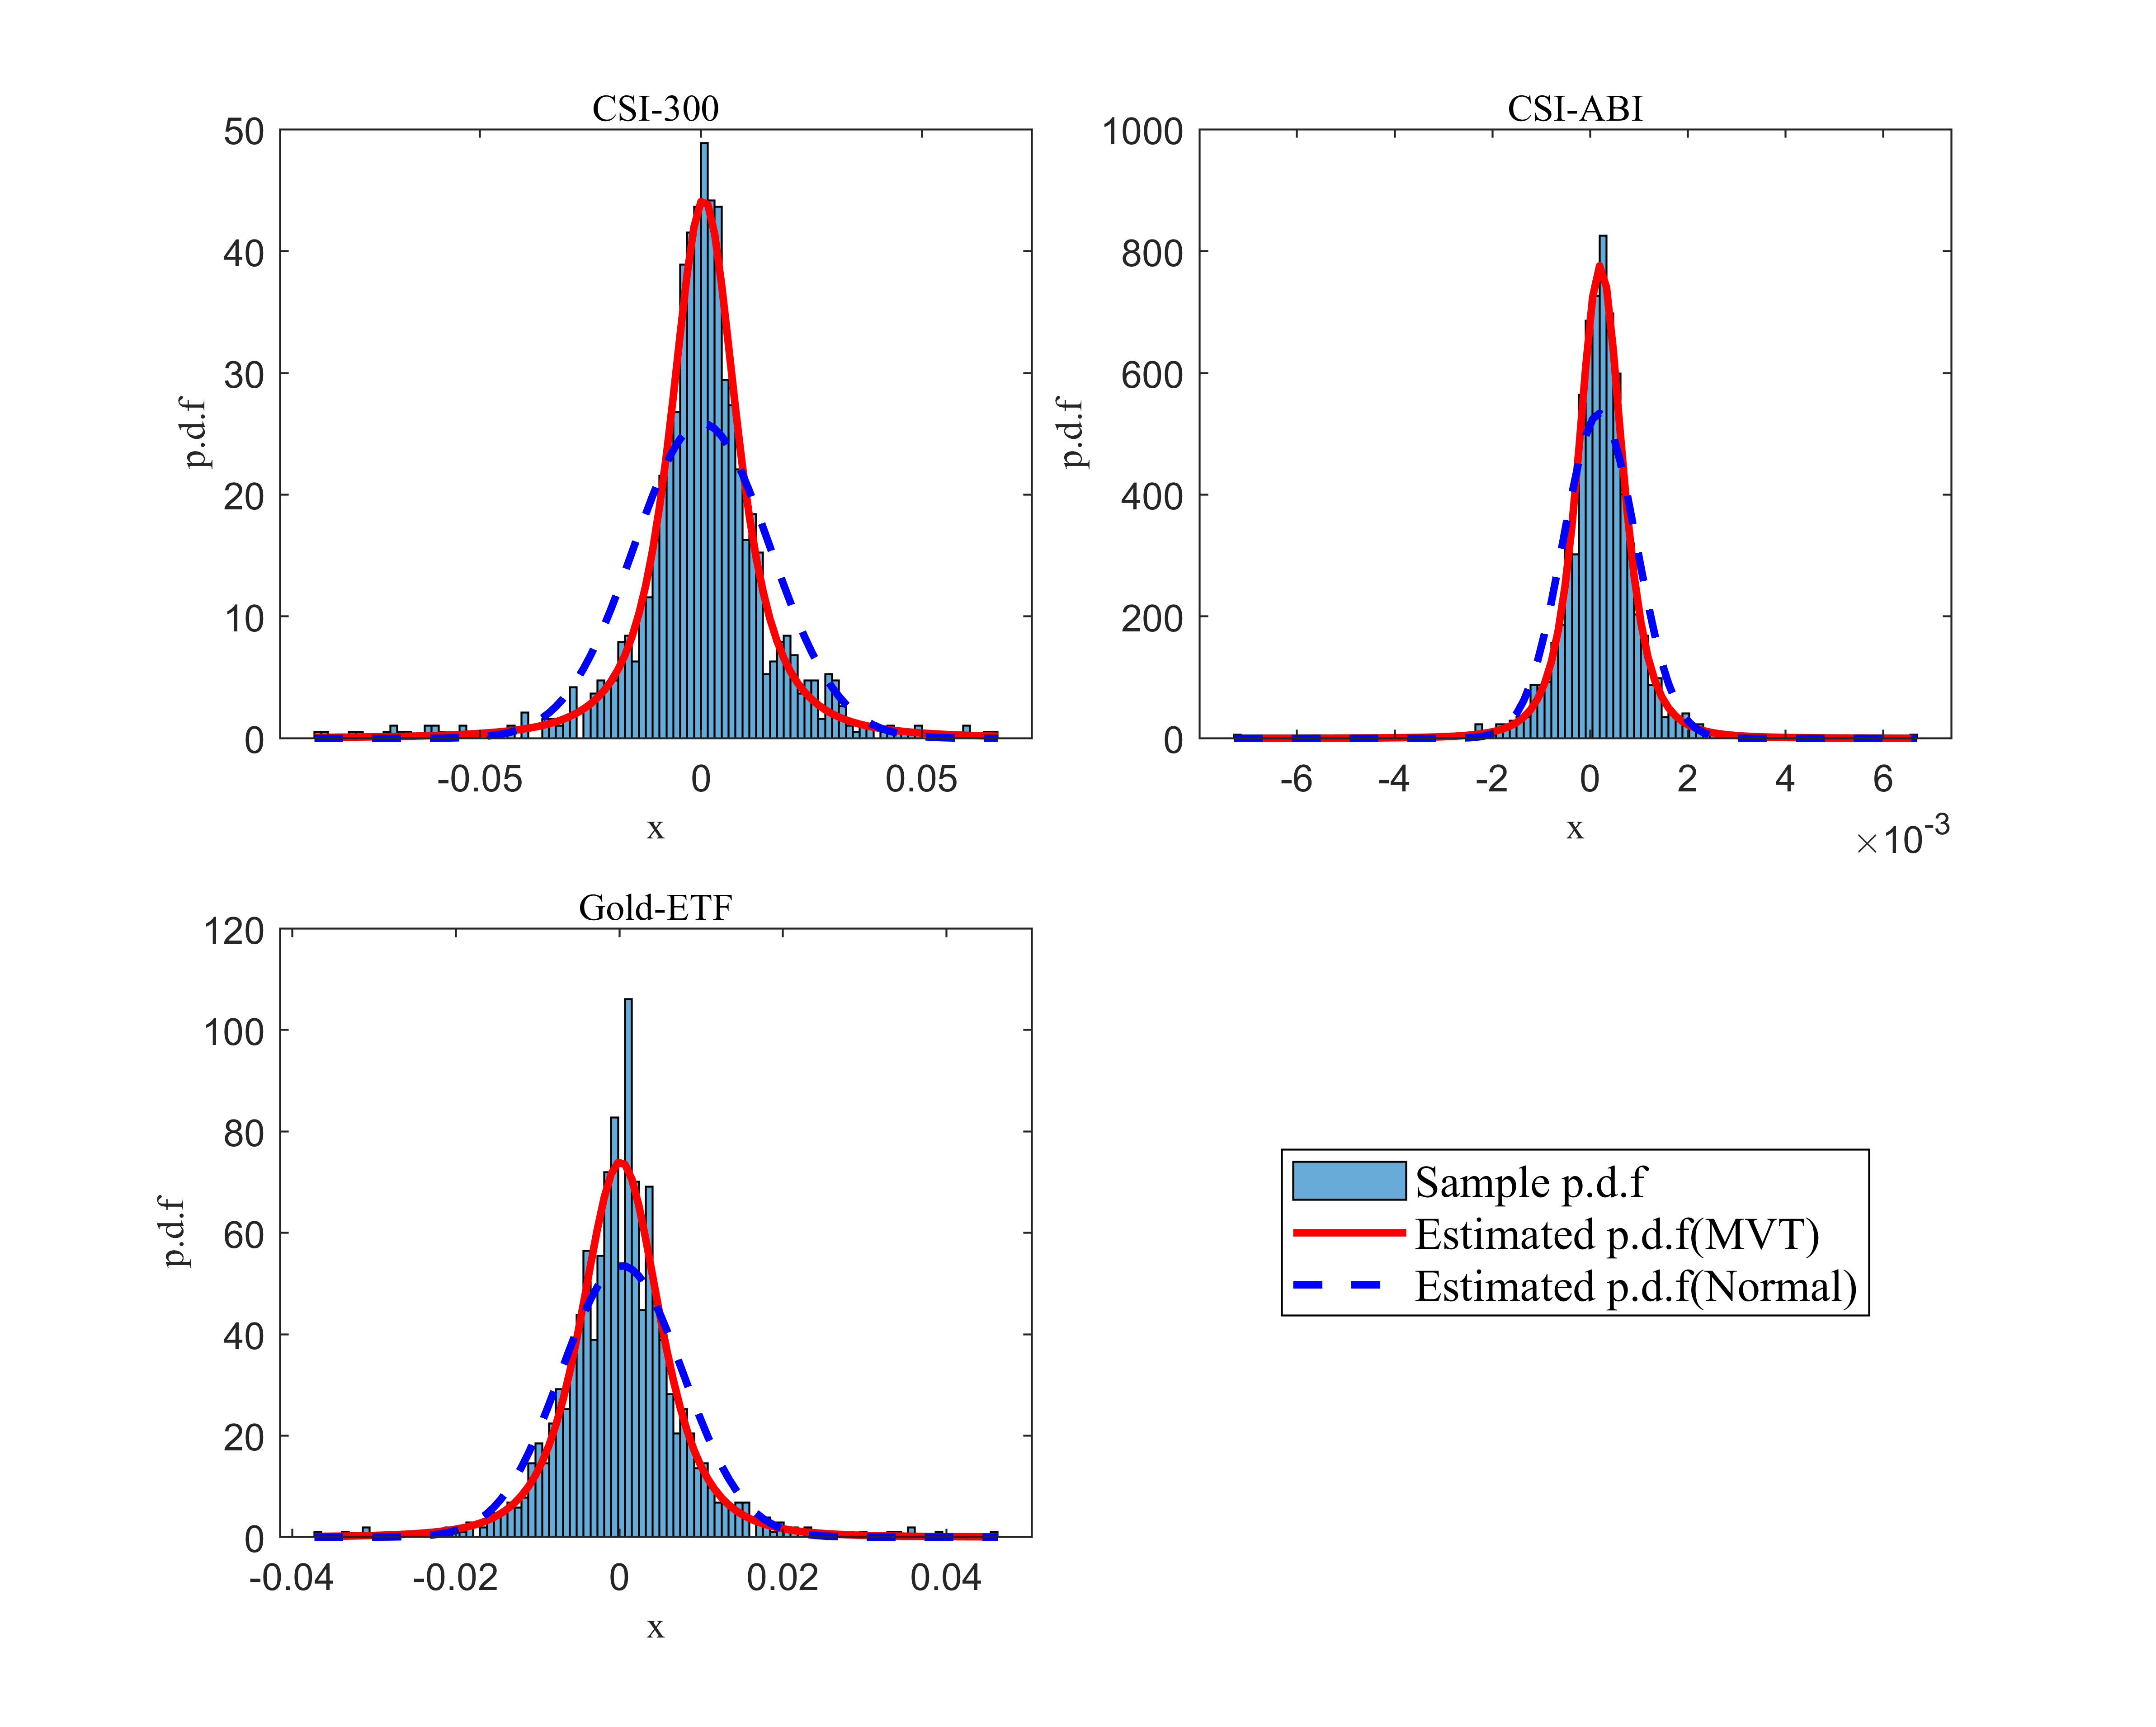
\includegraphics[scale=0.4]{Figure/FIG3-PDF.png}
    \label{Fig3}
\end{figure}
\end{frame}


\subsection{VaR and ES based on MVT}
\begin{frame}{VaR and ES based on MVT}

\begin{block}{Theoretical Formula}
Assume the return $r=(r_1,r_2,r_3)^T \sim t_{\nu}(\mu,\Sigma)$ is a 3-variate t-distribution random variable, then the return of a portfolio with weight $w=(w_1,w_2,w_3)^T$ is $r_p(w)=w^Tr \sim t_{\nu}(w^T\mu,w^T\Sigma w)$. 
\begin{equation} \label{E2.3}
\begin{aligned}
\text{VaR}_{\alpha}\left(r_p(w)\right) &= \mu_p(w) +\Sigma_p(w) t_{\nu}^{-1}(\alpha)    \\
\text{ES}_{\alpha}\left(r_p(w)\right) &= \mu_p(w) +\Sigma_p(w) \text{ES}_{\alpha}\left(t\right) \\
&=\mu_p(w) -\Sigma_p(w) \frac{f_{t_{\nu}}\left(t^{-1}_\alpha(\nu)\right)}{F_{t_{\nu}}\left(t^{-1}_\alpha(\nu)\right)} \cdot \frac{\left(\nu+(t^{-1}_\alpha(\nu))^2\right)}{\nu-1}
\end{aligned}
\end{equation}
where $\mu_p(w)=w^T\mu$ and $\sigma_p^2(w)=w^T\Sigma w$
\end{block}
\end{frame}

\begin{frame}{VaR and ES based on MVT} 
To compare the estimation effect of risk measurement based on MVT and normal distribution, we construct the Monte Carlo Simulation.
\begin{figure}[H]
    \centering
    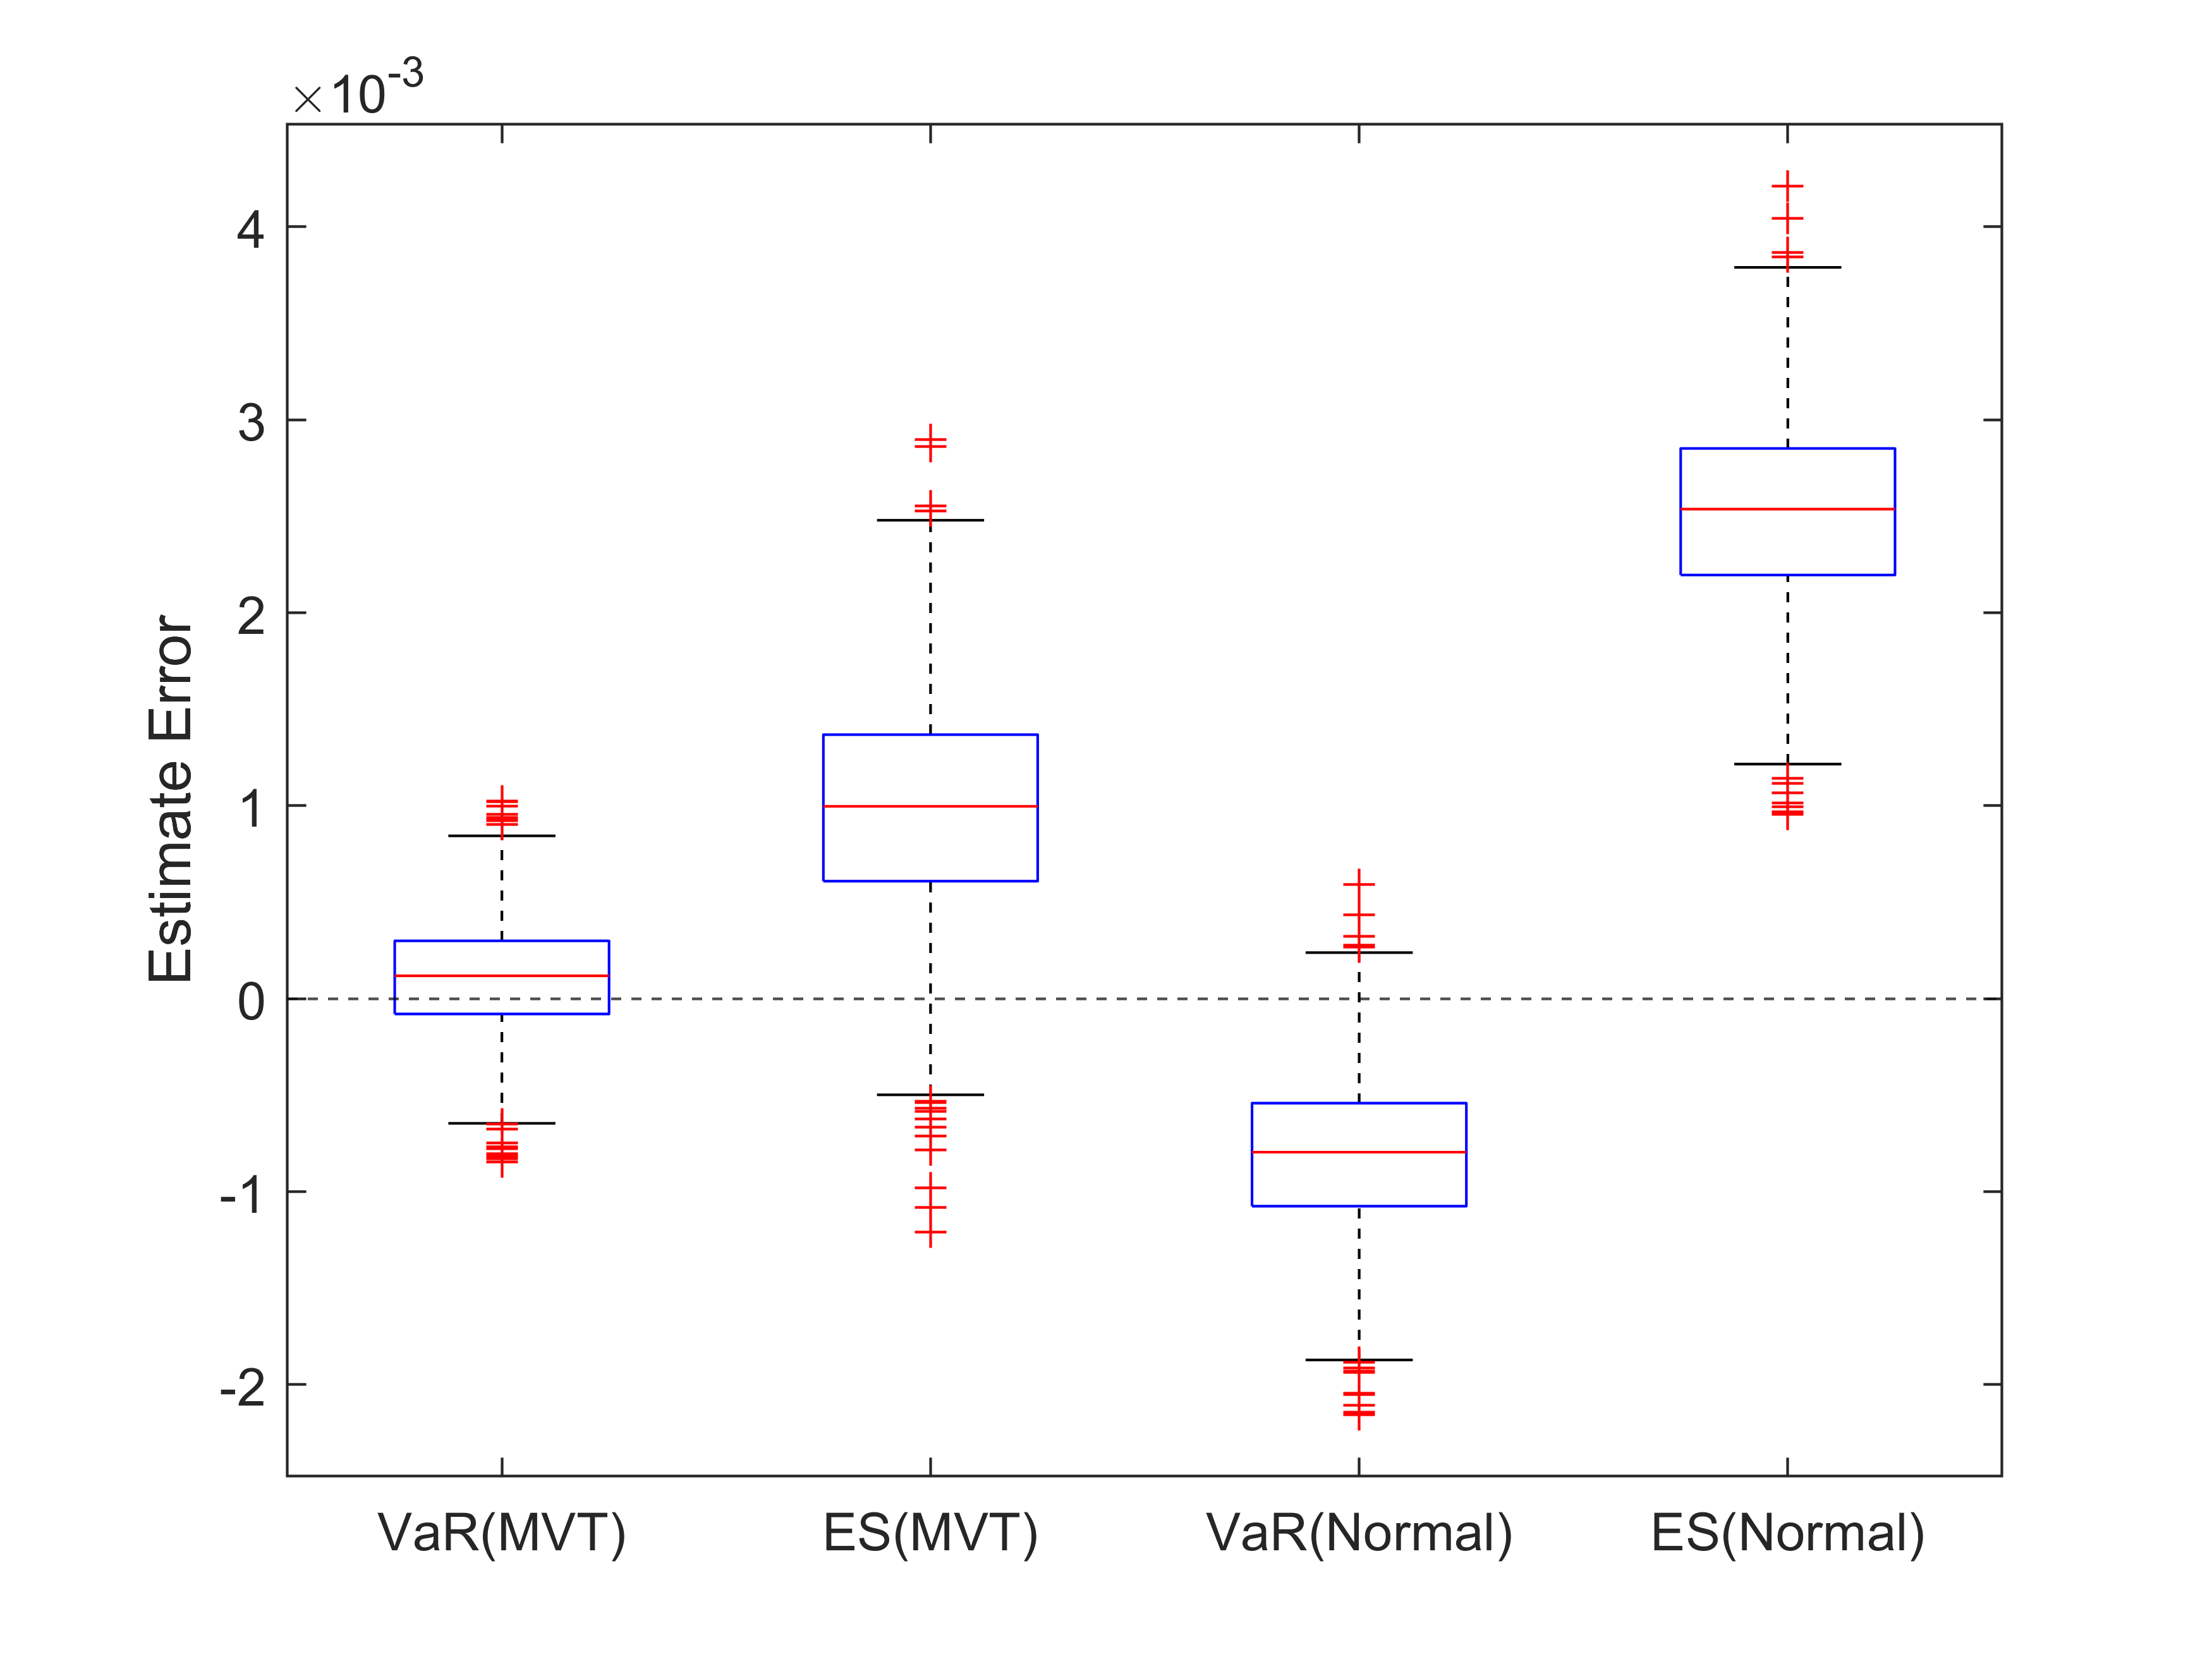
\includegraphics[scale=0.5]{Figure/FIG4-MC.png}
    \label{Fig4}
\end{figure}



\end{frame}



\section{Risk Parity Model Based on MVT}
\begin{frame}

\frametitle{Overview} % Table of contents slide, comment this block out to remove it
\tableofcontents[currentsection] % Throughout your presentation, if you choose to use \section{} and \subsection{} commands, these will automatically be printed on this slide as an overview of your presentation
\end{frame}

\subsection{Data Selection}
\begin{frame}
In order to test whether the risk parity model based on MVT can perform well in the actual market.
\frametitle{Data Selection}
\begin{itemize}
    \item We construct the risk parity model for CSI 300, CSI ABI and Gold ETF and carry out the dynamic backtesting.
    \item In terms of the time duration, we still applied the logarithmic rate of return data from 2015 to 2019.
    \item However, due to the need to estimate parameters and calculate risk metrics during the backtesting process, the actual backtesting interval is from April 2015 to December 2019.
\end{itemize}
\end{frame}

\subsection{Model Derivation}
\begin{frame}{Model Derivation}
The risk measure $\boldsymbol{\mathcal{R}}(.)$ is a mapping from $\mathcal{F}$ to space $\mathbb{R}$. The risk measure is consistent if it satisfies the following properties: 
\begin{block}{Consistency in Risk Metrics}
\begin{itemize}
  \item Monotonicity: $\forall X_1 \geq X_2 \in \mathcal{F}, \mathcal{R}\left(\mathrm{X}_1\right) \geq \mathcal{R}\left(\mathrm{X}_2\right)$ 
  \item Homogeneity: $\forall X \in \mathcal{F}, c \geq 0, \mathcal{R}(\mathrm{cX})=c \mathcal{R}(\mathrm{X})$
  \item Translation Invariance: $\forall X \in \mathcal{F}, c \in \mathbb{R}, \mathcal{R}(\mathrm{X}+\mathrm{c})=\mathcal{R}(\mathrm{X})-c$ 
  \item Subadditivity: $\forall X_1, X_2, \ldots, X_N \in \mathcal{F}, \mathcal{R}\left( \sum_{i=1}^{N} X_i\right) \leq \sum_{i=1}^{N} \mathcal{R}\left(X_i\right)$
\end{itemize}
\end{block}  
\end{frame}

\begin{frame}[t]{Model Derivation}
\begin{block}{Model Extension}
\begin{itemize}
    \item \textbf{Model based on Standard Deviation}
    \begin{equation*}
     \boldsymbol{\mathcal{R}}\boldsymbol{C}\left(X_i\right)=w_i \frac{\partial \boldsymbol{\mathcal{R}}_{\boldsymbol{p}}}{\partial w_i}=w_i \frac{(\Sigma \vec{w})_i}{\sqrt{\vec{w}^T \sum \vec{w}}}  
    \end{equation*}
    \item \textbf{Model based on $\text{VaR}_{\boldsymbol \alpha}$}
    \begin{equation*}
     \boldsymbol{\mathcal{R}}\boldsymbol{C}\left(X_i\right)=-w_i\mu_{i} - w_i \frac{(\Sigma \vec{w})_i}{\sqrt{\vec{w}^T \sum \vec{w}}}t_{\nu}^{-1}(\alpha)  
    \end{equation*}
    \item \textbf{Model based on $\text{ES}_{\boldsymbol \alpha}$}
    \begin{equation*}
     \boldsymbol{\mathcal{R}}\boldsymbol{C}\left(X_i\right)=-w_i\mu_{i} + w_i \frac{(\Sigma \vec{w})_i}{\sqrt{\vec{w}^T \sum \vec{w}}}\frac{f_{t_{\nu}}\left(t^{-1}_\alpha(\nu)\right)}{F_{t_{\nu}}\left(t^{-1}_\alpha(\nu)\right)} \cdot \frac{\left(\nu+(t^{-1}_\alpha(\nu))^2\right)}{\nu-1} 
    \end{equation*}
\end{itemize}
\end{block}  
\end{frame}

\subsection{Model Backtesting}
\begin{frame}{Model Backtesting}
We use the method of quarterly rebalancing for backtesting. There are 1, 2, ..., 19 quarters in total. When repositioning for time $t$, the following steps are performed:
\begin{enumerate}
    \item Calculate the parameters of MVT and the risk measures each asset in the $ t^{th}$ quarter.
    \item Use the risk parity model to calculate the weight of each asset $w_{t} = (w_{1}, w_{2}, w_{3} )^{T}$ in period t.
    \item Calculate the indicators used to evaluate the performance of the models.
\end{enumerate}
\end{frame}

\subsection{Result Analysis}
\begin{frame}{Result Analysis}
The following table shows the evaluation indexes of models and assets from Apr,2015 to Dec,2019 under the condition of $R_f=3\%$.
\begin{table}[H]
    \centering
   \begin{tabular}{|c|c|c|c|c|}
    \hline
    {Index} & {Annual Return} &  {Std} &  {MDD} & {Sharp Ratio}  \\
    \hline
    {std Model} &     5.39\% &     1.83\% &     4.00\% &    1.3080    \\
    \hline
    {VaR Model} &     5.25\% &     1.71\% &     3.94\% &    1.3157   \\
    \hline
    {ES Model} &     5.28\% &     1.73\% &     3.94\% &    1.3161   \\
    \hline
    {CSI 300} &     0.23\% &    23.86\% &    61.71\% &   -0.1159    \\
    \hline
    {CSI ABI} &     4.81\% &     1.15\% &     4.47\% &    1.5745   \\
    \hline
    {GOLD ETF} &     7.79\% &    11.50\% &    15.64\% &    0.4167  \\
    \hline
    \end{tabular}  
    \label{Tab3}
\end{table}
\end{frame}

\begin{frame}{Result Analysis}
The following figure shows that the weight of assets based on Std Model, VaR Model, and ES Model respectively.
\begin{figure}[H]
    \centering
    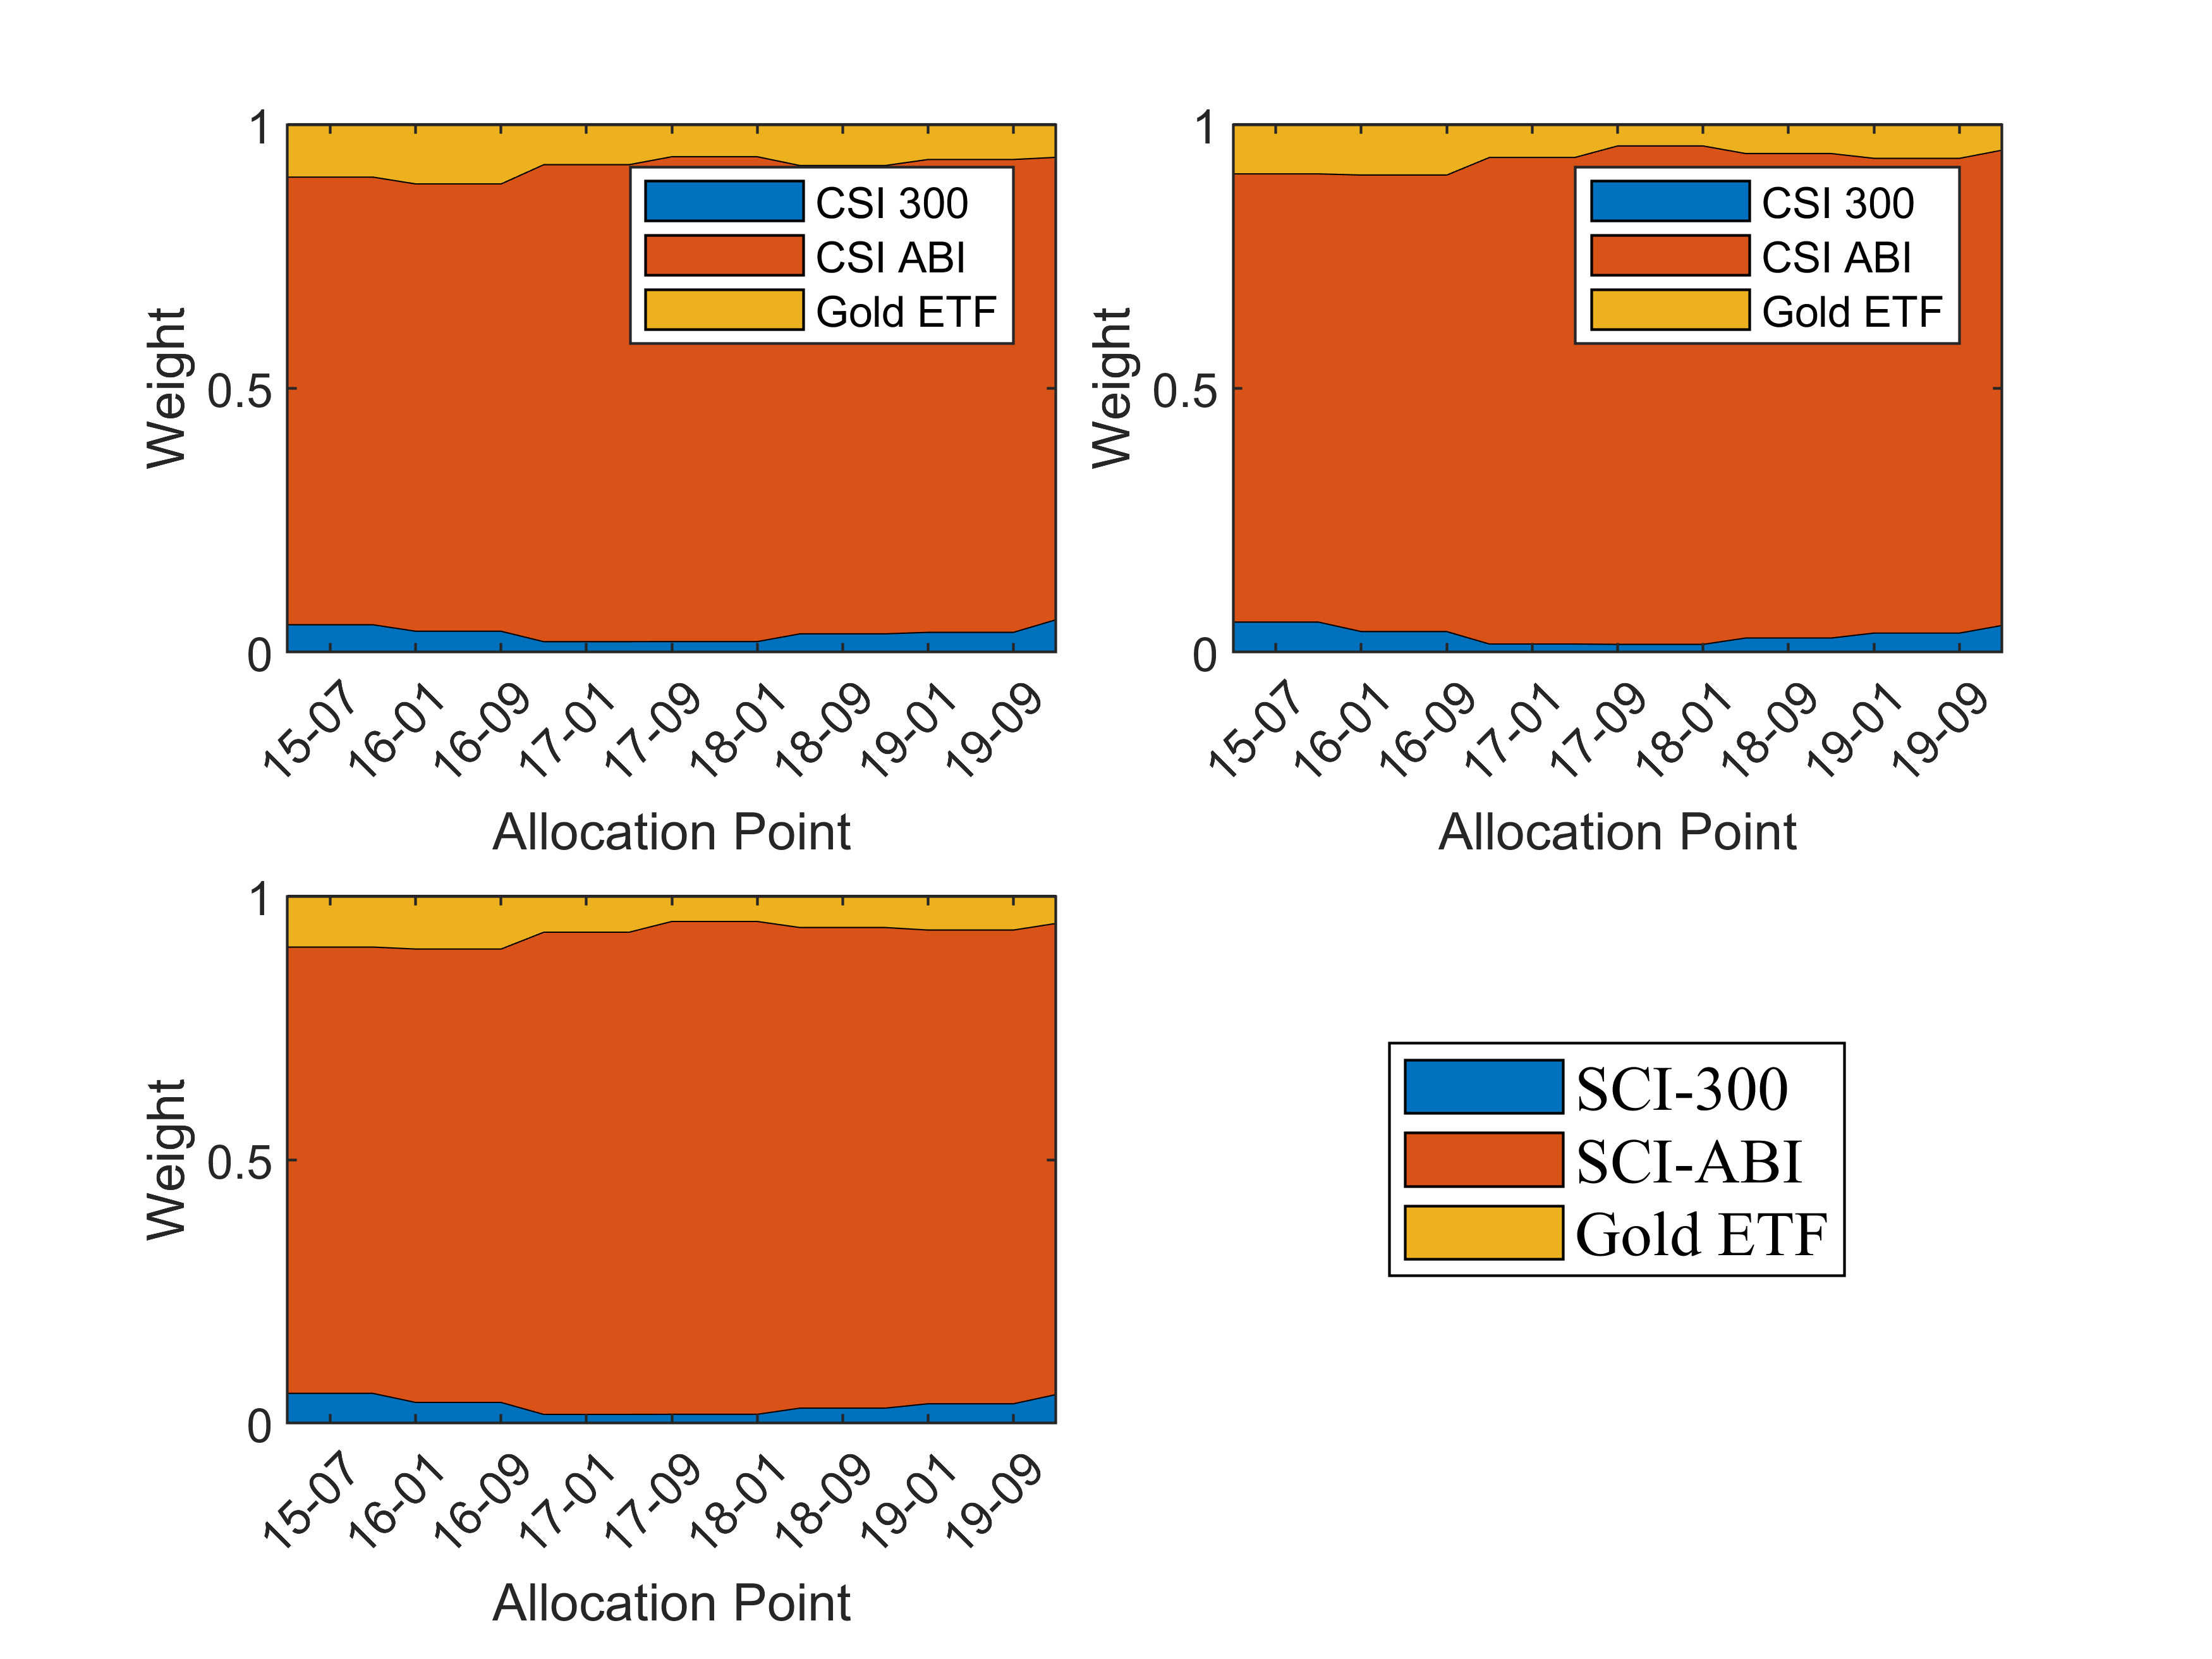
\includegraphics[scale=0.5]{Figure/FIG5-Allocation_Weight.png}
    \label{Fig5}
\end{figure}
\end{frame}

\begin{frame}{Result Analysis}
\begin{enumerate}
    \item \textbf{Allocation Models All Outperform Individual Assets}
    \begin{itemize}
        \item The annualized rate of return is higher than that of CSI 300 and CSI ABI, and lower than gold ETF.
        \item The annualized volatility is much lower than that of CSI 300 and gold ETF, while it is slightly higher than that of CSI ABI.
        \item Sharpe ratio is significant higher than that of a single asset.
    \end{itemize}
    \item \textbf{Different Models Have Their Own Characteristics}
        \begin{itemize}
        \item Compared with the standard deviation models, the performance of the VaR model and the ES model is basically the same.
        \item With respect to the Sharpe ratio, the standard deviation model is the lowest and the expected shortfall model is the highest.
    \end{itemize}
    \item \textbf{Weight Allocation with More Debt and Less Shares}
        \begin{itemize}
        \item The average allocation ratio of the VaR model is the lowest in the CSI 300 Index and the gold ETF, and the highest in the CSI ASI.
        \item The expected shortfall model is more sensitive to the changes of the upward and downward trend.
        \item The asset allocation ratio has more bonds than stocks.
        \end{itemize}
\end{enumerate}
\end{frame}

\begin{frame}
\frametitle{References}
\footnotesize{
\begin{thebibliography}{99} % Beamer does not support BibTeX so references must be inserted manually as below
\bibitem [Artzner, Philippe, e. a. (1999)]{p1} Artzner, Philippe, e. a. (1999). Coherent measures of risk. Mathematical finance, pages 203–228
\bibitem[Bawa, V. S. (1975)]{p1} Bawa, V. S. (1975). Optimal rules for ordering uncertain prospects. Journal of Financial Economics, pages 95–121.
\bibitem[Hasannasab, M., Hertrich, J., Laus, F., and Steidl, G. (2021)]{p1} Hasannasab, M., Hertrich, J., Laus, F., and Steidl, G. (2021). Alternatives to the EM algorithm for ML estimation of location, scatter matrix, and degree of freedom of the student t distribution. Numerical Algorithms, 87(1):77–118.
\bibitem[Markowitz, H. M. (1991)]{p1} Markowitz, H. M. (1991). Foundations of portfolio theory. The journal of finance, pages 469–477.
\bibitem[Qian, E. (2005)]{p1} Qian, E. (2005). Risk parity portfolios: Efficient portfolios through true diversification
(investment insight). page to appear.
\bibitem[Rockafellar R T, U. S. (2002)]{p1} Rockafellar R T, U. S. (2002). Conditional value-at-risk for general loss distributions.
Journal of banking $\&$ finance, pages 1443–1471.
\bibitem[Tasche, D. (2002)]{p1} Tasche, D. (2002). Expected shortfall and beyond. Journal of Banking $\&$ Finance, pages 1519–1533.
\end{thebibliography}
}
\end{frame}


\begin{frame}
\Huge{\centerline{The End}}
\end{frame}

%----------------------------------------------------------------------------------------


\end{document}